\subsection{Extreme Spatial Scaling}

Figure \ref{fig:extreme-nx} presents an extreme spatial scaling test, pushing the grid resolution (\(N_x\)) from 1,000 up to 100,000 elements at a strict \(10^{-6}\) tolerance. The simulation time is fixed at \(T=0.05\) and the index \(p = 2.5\). This test aims to bottleneck the solvers primarily at the hardware memory and linear algebra level, seeking to minimize the relative impact of the inherent overhead from their respective Python wrappers.

Both solvers exhibit highly predictable, near-linear scaling on a log-log scale as the grid grows. For the first half of the parameter sweep (\(N_x \le 25,000\)), LSODA maintains a distinct performance lead. For instance, at \(N_x = 25,000\), LSODA completes the integration in 12.69 seconds, whereas CVODE finishes in 21.21 seconds. This suggests that at small to intermediate spatial scales, the structural and memory-mapping overhead of the SUNDIALS wrapper likely introduces a computational drag.

Around \(N_x = 50,000\), the performance trajectories temporarily converge, with CVODE barely edging out LSODA (finishing in 39.20 seconds compared to LSODA's 39.70 seconds). This brief crossover points to a potential shift in the system's computational bottleneck; at this scale, the memory footprint of the tridiagonal system and the cost of the internal sparse LU factorizations appear to dominate the hardware resources.

However, at the upper limit of the sweep (\(N_x = 100,000\)), LSODA regains its advantage, completing the simulation in 138.88 seconds while CVODE takes 152.36 seconds. Despite CVODE's optimized C-level sparse linear algebra backend, SciPy's LSODA remains remarkably competitive and seemingly more efficient in this specific configuration even when the system's memory bandwidth is heavily taxed.

\begin{figure}[H]
  \centering
  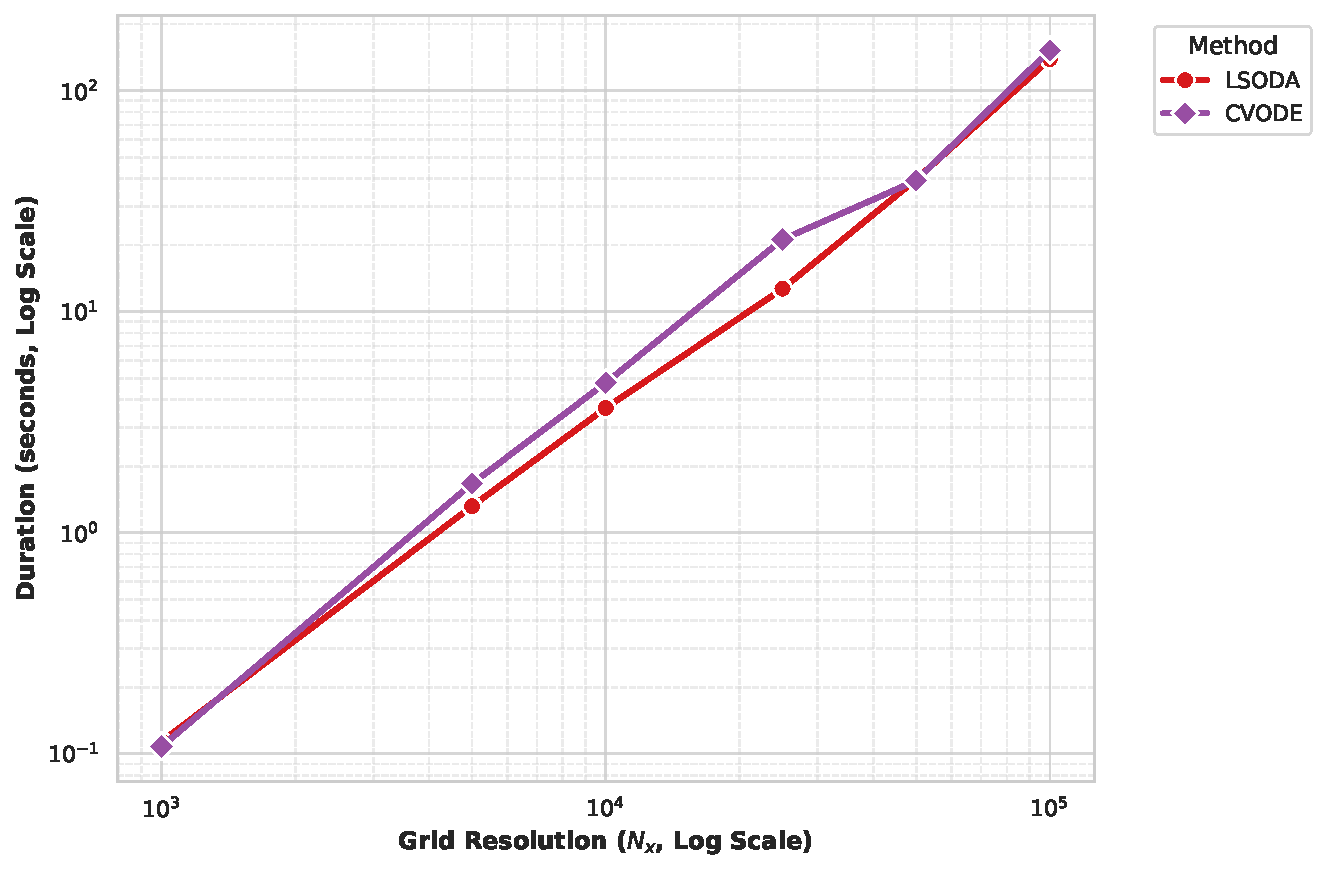
\includegraphics[width=\textwidth]{images/extreme_nx_scaling.pdf}
  \caption{Execution time scaling for LSODA and CVODE across massive spatial grid resolutions (\(N_x = 1000\) to \(100,000\)).}
  \label{fig:extreme-nx}
\end{figure}
